\subsection{Aufgabe 1: HTML}
\label{sec:Aufgabe1}
\begin{enumerate}[label=\alph*)]
    \item Was ist ein Pseudoelement? (\textbf{multiple chioce})
    \item Wie sehen Kommentare in HTML? (\textbf{multiple chioce})
    \item Welche Sonderzeichen müssen in der URL ersetzt werden? (\textbf{multiple chioce})
        \begin{enumerate}[label=\arabic*.]
        \item =
        \item \#
        \item ?
        \item \%
        \end{enumerate}
    \item Wie sieht der zugehörige HTML-Code aus? \\
        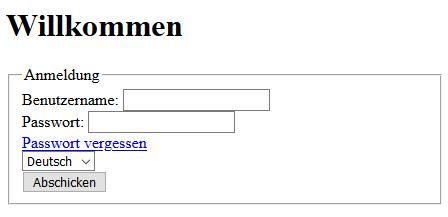
\includegraphics[width=15cm]{img/klausur.JPG}
        \begin{enumerate}[label=\arabic*.]
                % use '' instead of " because "o -> ö etc. in babel package.
            \item Die Parameter sollen als ''benutzername'', ''passwort'' und
                ''sprache'' beim Server abfragbar sein.
            \item Benutzername ist max. 80 Zeichen lang und muss immer angegeben werden.
            \item Passwort soll nicht lesbar sein.
            \item Passwort vergessen leitet nach ''/passwortzuruecksetzen'' weiter.
            \item Sprache Deutsch soll standardmäßig aktiv sein. Die andere Option
                ist Englisch.
            \item Das Formular soll an ''/auswertung.php'' geschickt werden und
                POST ausgelesen werden können.
         \end{enumerate}
    \item Nennen Sie 4 Statuscodes und erläutern Sie kurz ihre Bedeutung.
    \item Nennen Sie 4 HTTP Methoden und erläutern Sie kurz ihre Bedeutung.
\end{enumerate}
